\subsection{An audit that uses observed fields without conditional-mean labels}
To test \Cref{thm:observed-audit,thm:dependency}, use the sine basis above with
\begin{equation}\label{eq:bounded-observed-field}
 U_1=X,\qquad U_j=\frac{m(X)+0.1\xi_j}{j}\quad(j\ge2),\qquad
 m(x)=0.7\tanh(0.8x)+0.1\sin(3x),
\end{equation}
where $X,\xi_2,\ldots$ are independent uniform variables on $[-1,1]$.
The first coefficient is a sufficient context for every later band. The target mean obeys $|m|\le0.8$ and $\Lip(m)\le0.86$. The target tail satisfies
$\tau_m^2\le(0.8^2+0.1^2/3)\sum_{j>m}j^{-2}$.

Three networks, with seeds $481,482,483$, each have twelve slopes and twelve softmax weights:
$f_\theta(x)=\sum_{k=1}^{12}p_k\tanh(a_kx)$.
The slopes are constrained to $[-1.3,1.3]$, giving the exact implemented sensitivity $\sum_kp_k|a_k|$. Each network trains on $16{,}384$ noisy fields through eight modes, using $1{,}200$ Adam steps and batches of $1{,}024$ randomly chosen field-mode pairs. The regression target is the observed normalized coefficient $jU_j$, not $m(X)$. Generation uses $(f_\theta(X)+0.1\xi_j)/j$. A fourth, predeclared candidate has $f=0$. All candidates share the known noise scale; learning an unspecified noise law would require a different model fit, although the distributional audit itself can compare more general scalar laws.

Two independent audit splits use seeds $7401,7402$. For budgets $n=4{,}096$, $16{,}384$, and $65{,}536$ fields per split, the feature partitions have respectively eight, twelve, and sixteen equal cells. These choices are fixed before the audit; the total failure budget $0.01$ is divided across the three budgets. Within each budget, the union bounds cover all four candidates and all 31 audited detail bands, hence every retained cutoff. Dependence between modes of one field is allowed. No cell is empty in the realized datasets; the code nevertheless implements the diameter bound for empty cells.

Both target and learned normalized details lie in $[-1.1,1.1]$. The empirical-to-model transport has a closed formula. For sorted observations $z_{(i)}$, $i=1,\ldots,n$, and a uniform model on $[c-\sigma,c+\sigma]$,
\begin{equation}\label{eq:empirical-uniform}
 W_2^2\!\left(\frac1n\sum_i\delta_{z_i},\operatorname{Unif}[c-\sigma,c+\sigma]\right)
 =\frac1n\sum_i\left[z_{(i)}-c-\sigma\left(\frac{2i-1}{n}-1\right)\right]^2
 +\frac{\sigma^2}{3n^2}.
\end{equation}
This follows by integrating the squared difference of the two quantile functions on each interval of length $1/n$. Thus the audit evaluates observed detail distributions against the learned kernel directly. It receives the support and regularity assumptions but never calls the target-mean function. Floating-point evaluation of the formula is kept distinct from a formally rounded numerical enclosure.

Because the sole parent coordinate is sampled exactly, \Cref{thm:dependency} combines the certified fitting inputs in quadrature. For seed 481 at $m=32$ and the largest budget, the generic prefix recurrence gives $0.908405$, whereas the dependency certificate gives $0.585551$. This improvement uses a proved architectural restriction, not a smaller confidence budget. Across all three trained seeds the latter bound ranges from $0.585268$ to $0.587704$. The no-context bound is $0.723932$.

\begin{table}[htbp]
\centering\small
\begin{tabular}{rrrrr}
\toprule
Fields per split & Cells & Learned bound & No-context bound & Coupling upper \\
\midrule
4,096 & 8 & 1.0304 & 1.0632 & 0.0633 \\
16,384 & 12 & 0.7653 & 0.8687 & 0.0633 \\
65,536 & 16 & 0.5856 & 0.7239 & 0.0633 \\
\bottomrule
\end{tabular}

\caption{Observed-data certification at 32 modes. The learned columns use the predeclared seed 481. Every bound includes a justified infinite target tail and belongs to the simultaneous 99\% event. The final column is a separate numerical evaluation of a specified full-law coupling, using the synthetic truth only for this diagnostic; it is not the audit input or an optimal transport distance.}\label{tab:observed-audit}
\end{table}
\begin{figure}[htbp]
\centering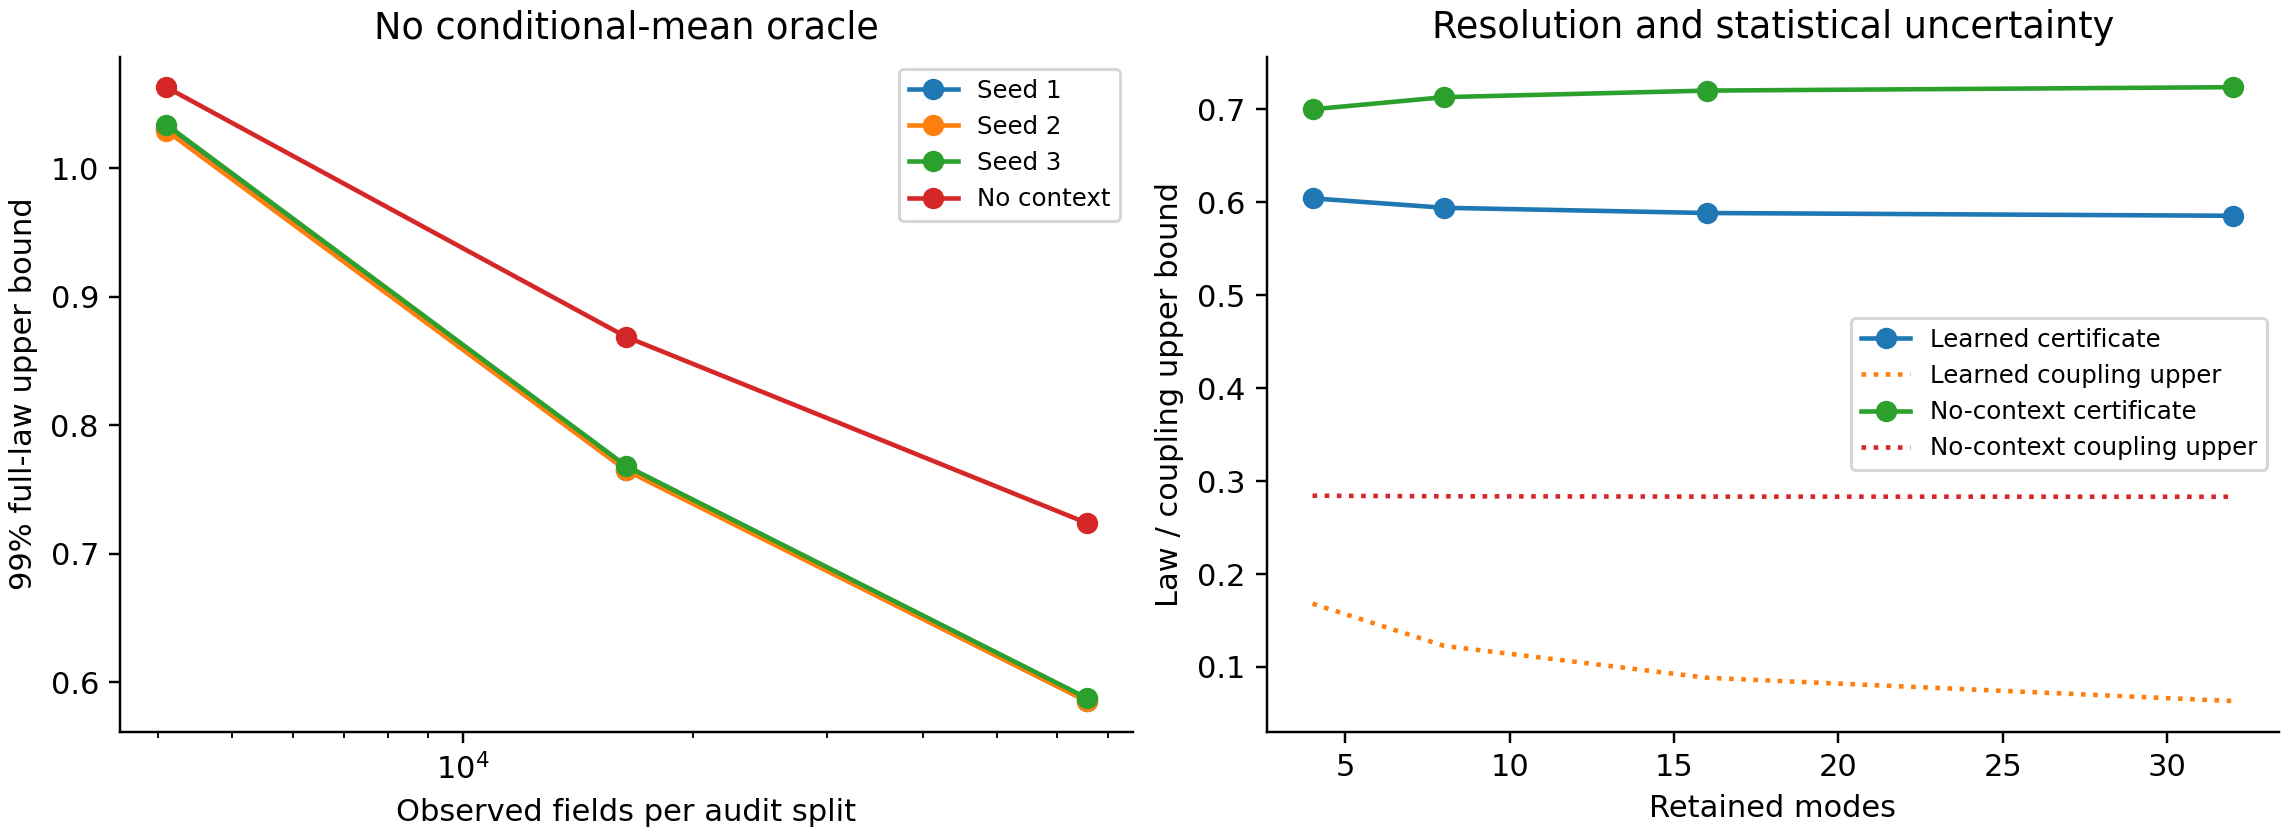
\includegraphics[width=\textwidth]{figures/observed_audit.png}
\caption{Observed-data audit with two independent splits. Left: all three trained seeds and the no-context candidate. Right: the dependence on retained resolution at the largest budget. Dotted lines evaluate a specified coupling using the known synthetic law; solid lines include statistical uncertainty and the deterministic tail envelope.}\label{fig:observed-audit}
\end{figure}

The actual conditional mean discrepancy is evaluated only in a separate truth diagnostic. Sharing $X$ and every uniform innovation makes each retained detail discrepancy $(m(X)-f_\theta(X))/j$. A 512-point Gauss--Legendre integral computes its squared mean; repeating with 1,024 points changes it by less than $10^{-15}$. For seed 481, the resulting full-law coupling upper estimate at 32 modes is $0.0633$. The much larger statistical certificate exposes the price of distribution-free cellwise estimation, the support envelope, and simultaneous coverage. The bound is informative as a guaranteed radius under the assumptions, but is not a precise estimator of the attained error. The target's analytic tail envelope also exceeds its actual tail. The code records both the generic and dependency recursions, every bandwise confidence input, cell occupancy, and all trained parameters.

\subsection{A geometry check for overlapping coordinates}
\Cref{fig:observation-geometry} evaluates the exact two-coordinate example in \Cref{sec:riesz}. The aligned discrepancy $x=y$ has squared physical-to-coordinate error ratio $1+c$, while the encoder's condition number is $\sqrt{(1+c)/(1-c)}$. The two quantities answer different questions: the former transfers a forward approximation bound, and the latter measures the worst relative instability of recovering coordinates. The plot checks the analytic formulas; it is not a fitted neural experiment.
\begin{figure}[htbp]
\centering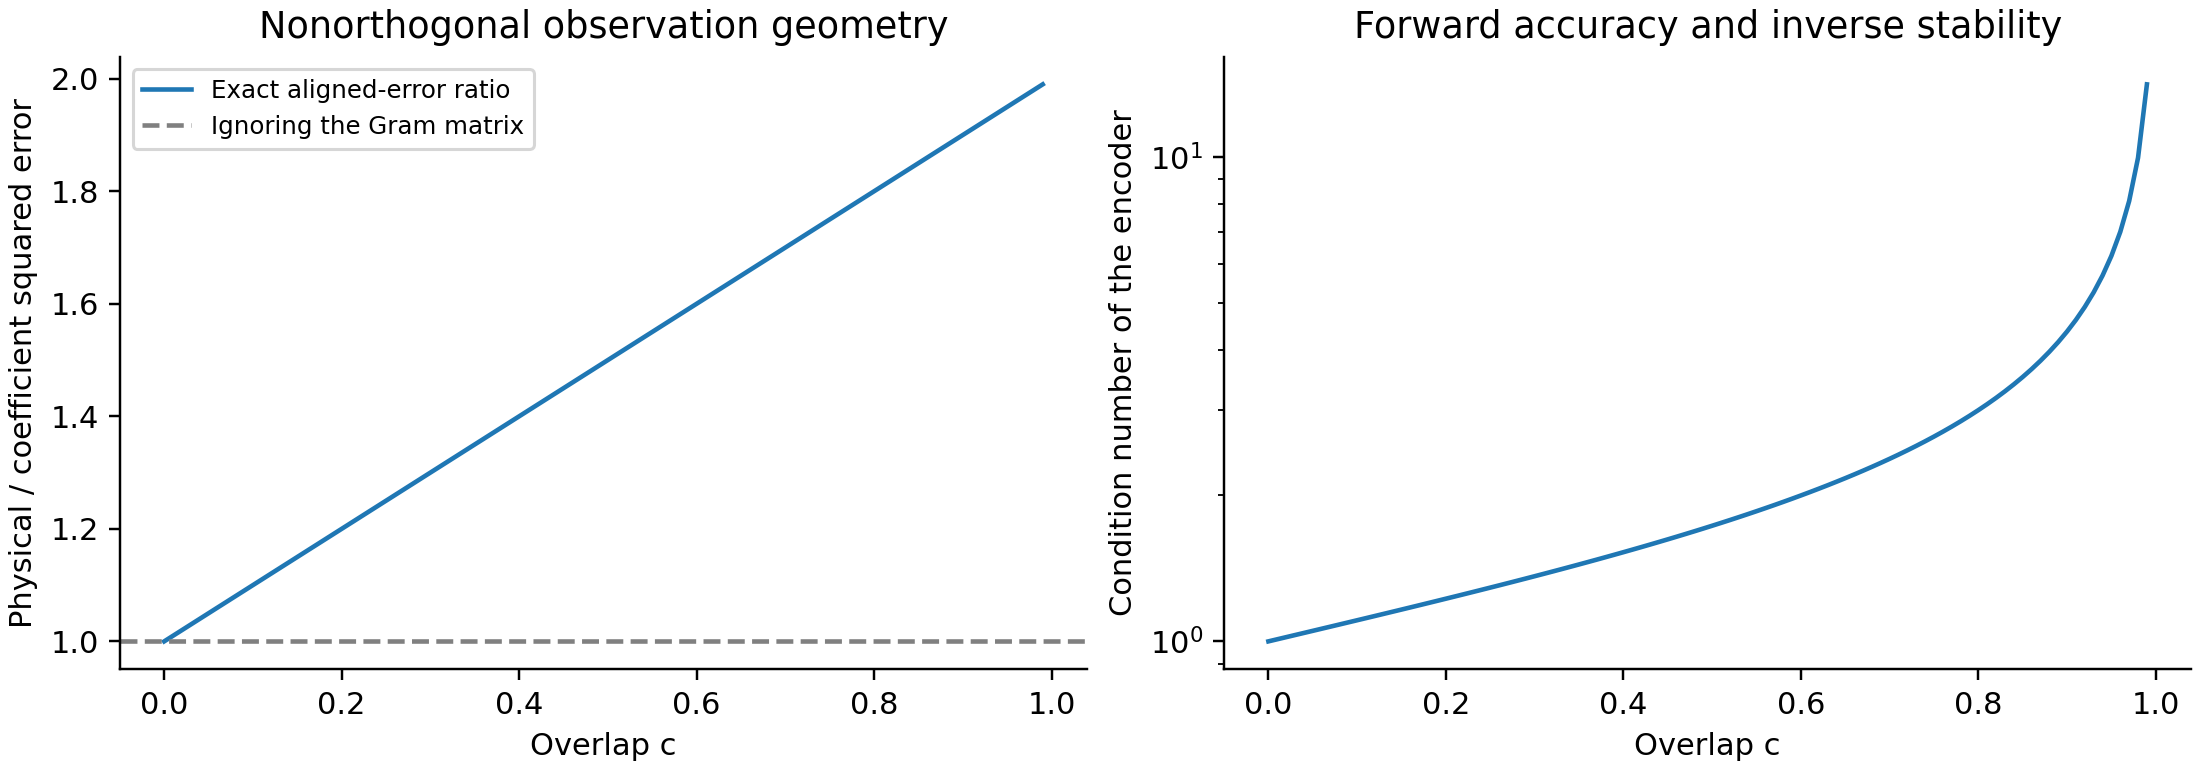
\includegraphics[width=\textwidth]{figures/observation_geometry.png}
\caption{Overlapping observation coordinates. Forward error distortion can remain bounded while the inverse representation becomes arbitrarily ill-conditioned.}\label{fig:observation-geometry}
\end{figure}
